\documentclass{beamer}
%
% Choose how your presentation looks.
%
% For more themes, color themes and font themes, see:
% http://deic.uab.es/~iblanes/beamer_gallery/index_by_theme.html
%
\mode<presentation>
{
  \usetheme{default}      % or try Darmstadt, Madrid, Warsaw, ...
  \usecolortheme{crane} % or try albatross, beaver, crane, ...
  \usefonttheme{structurebold}  % or try serif, structurebold, ...
  \setbeamertemplate{navigation symbols}{}
  \setbeamertemplate{caption}[numbered]
} 

\usepackage[english]{babel}
\usepackage[utf8x]{inputenc}

\usepackage{tikz}

\newcommand{\C}{\mathbb{C}}
\newcommand{\R}{\mathbb{R}}
\newcommand{\cC}{\mathcal{C}}
\newcommand{\cD}{\mathcal{D}}
\renewcommand{\>}{\rangle}
\newcommand{\<}{\langle}

\title[Partition functions]{Simpler classical and faster quantum algorithms for Gibbs partition functions}
\author{Pawe{\l} Wocjan}
\institute{IBM Quantum, IBM T.J. Watson Research Center}
\date{IBM -- Tufts University Quantum Workshop\\July 2022}

\begin{document}

\begin{frame}
  \titlepage
\end{frame}

\begin{frame}{Simpler classical and faster quantum algorithms for Gibbs partition functions}
    Research project conducted by the Quantum Algorithms Group:
    
    \medskip
    \begin{itemize}
        \item Srinivasan Arunachalam
        \item Vojtech Havlicek
        \item Giacomo Nannicini
        \item Kristan Temme
        \item Pawel Wocjan
    \end{itemize}
\end{frame}

% Uncomment these lines for an automatically generated outline.
%\begin{frame}{Outline}
%  \tableofcontents
%\end{frame}

\section{Estimating partition functions}

\begin{frame}{Problem}
\begin{itemize}
    \item We consider the problem of approximating the partition function of a classical Hamiltonian using simulated annealing.
    
    \medskip
    \item This requires 
    
    \medskip
    \begin{itemize}
        \item (a) the computation of a cooling schedule
        
        \medskip
        \item (b) the ability to estimate the expectations of random variables that depend on Gibbs distributions at the inverse temperatures of the cooling schedule.
    \end{itemize}
\end{itemize}
\end{frame}

%

\begin{frame}{Accomplishments}
  \begin{itemize}
    \item We propose classical and quantum algorithms for these two tasks, achieving two goals: 
    
    \medskip
    \begin{itemize}
        \item (i) we simplify the seminal work of \v{S}tefankovi\v{c}, Vempala and Vigoda (\emph{J.~ACM}, 56(3), 2009), improving their running time and almost matching that of the current classical state of the art; 
        
        \medskip
        \item (ii) we quantize our new simple algorithm, improving upon the best known quatum algorithm for computing partition functions of many problems, due to Harrow and Wei (SODA 2020). 
    \end{itemize}
    \end{itemize}
\end{frame}

%

\begin{frame}{Accomplishments}
\begin{itemize}
    \item The proposed quantum algorithm has two advantages over the classical algorithm: 
    
    \medskip
    \begin{itemize}
    \item it has quadratically faster dependence on the spectral gap of the Markov chains as well as the precision, and
    
    \medskip
    \item it computes a shorter cooling schedule, which matches the length conjectured to be optimal by \v{S}tefankovi\v{c}, Vempala and Vigoda. 
\end{itemize}

\bigskip
\bigskip
\item (The algorithm requires a fault-tolerant quantum computer.)
\end{itemize}
\end{frame}

%

\begin{frame}{Hamiltonians}
    \begin{itemize}
        \item The \textcolor{blue}{state space $\Omega$} is some finite set.
        
        \medskip
        \item A (classical) \textcolor{blue}{Hamiltonian $H$} is function that assigns an \textcolor{blue}{energy $H(x)$} to each state $x\in\Omega$.
        
        \medskip
        \item The possible energies are
        \begin{equation*}
            H(x)\in\{0,1,\ldots,n\}
        \end{equation*}
        
        where $n$ is a positive integer.
    \end{itemize}
\end{frame}

%

\begin{frame}{Partition functions}

\begin{itemize}
    \item An \textcolor{blue}{inverse temperature $\beta$} is a non-negative real number.
    
    \medskip
    \item The \textcolor{blue}{partition function at $\beta$} is
    \begin{equation*}
        Z(\beta) = \sum_{x\in\Omega} \exp\big(-\beta H(x)\big).
    \end{equation*}
    
    \item The partition function at inverse temperature $\beta_{\min}=0$ is
    \begin{equation*}
        Z(\beta_{\min}) = |\Omega|.        
    \end{equation*}
    
    \item What can we say about the complexity of computing the partition function $Z(\beta_{\max})$ at a large inverse temperature $\beta_{\max}$?
\end{itemize}

\end{frame}

%

\begin{frame}{Complexity of partition functions}
    \begin{itemize}
        \item In general, it is not possible to efficiently compute the exact value $Z(\beta_{\max})$ for large $\beta_{\max}$ since
        
        \begin{equation*}
            Z(\beta_{\max}) \approx a_0
        \end{equation*}
        
        \medskip
        $a_0$ is the number of states $x\in\Omega$ with $H(x)=0$.
    
        \medskip
        \item It is easy to construct Hamiltonians whose \textcolor{blue}{ground states} correspond to the \textcolor{red}{solutions of some NP-hard problems}.
    
        \medskip
        \item $\Longrightarrow$ The goal is to \textcolor{blue}{estimate} $Z(\beta_{\max})$.
    \end{itemize}

\end{frame}

%

\begin{frame}{Estimating partition functions}

\begin{itemize}
    \item Let $\varepsilon\in(0,1)$ be the \textcolor{blue}{error} parameter.
    
    \medskip
    \item We want to obtain an \textcolor{blue}{estimate $\hat{Z}(\beta_{\max})$} of $Z(\beta_{\max})$ such that
    
    \begin{equation*}
        (1 - \varepsilon) \cdot Z(\beta_{\max}) \, \le \,
        \hat{Z}(\beta_{\max}) \, \le \,
        (1 + \varepsilon) \cdot Z(\beta_{\max})
    \end{equation*}
    
    \medskip
    holds with high probability ($\ge \frac{3}{4})$.
\end{itemize}

\end{frame}

%

\begin{frame}{Estimating partition functions}

\begin{itemize}
    \item 
    Equivalently, the above condition is expressed as
    \begin{equation*}
        | Z(\beta_{\max}) - \hat{Z}(\beta_{\max}) | \le
        \varepsilon \cdot Z(\beta_{\max})
    \end{equation*}
    
    \medskip
    \item We say that $\hat{Z}(\beta_{\max})$ estimates $Z(\beta_{\max})$ with \textcolor{blue}{relative} error $\varepsilon$.
    
    \bigskip
    \item It is not enough to obtain an estimate with \textcolor{red}{additive} error.
\end{itemize}

\end{frame}

%

\begin{frame}{Methods and Tools}

\begin{itemize}
\item The algorithms rely on several methods and tools. 

\medskip
\item These methods and tools can be logically organized into:

\medskip
\begin{itemize}
    \item Monte Carlo method 
    
    (classical and quantum Chebyshev inequalities)

    \medskip
    \item Simulated annealing 
    
    (Gibbs distribution, cooling schedule, product estimators)

    \medskip
    \item Markov chains 
    (quantization of Markov chains)
    
\end{itemize}
\end{itemize}
\end{frame}

%

\begin{frame}{Monte Carlo method}
    \begin{itemize}
        \item The \textcolor{blue}{Monte Carlo method} refers to a collection of tools for estimating values through sampling and simulation.

    \end{itemize}
\end{frame}

%

\begin{frame}{Monte Carlo method}
    \begin{itemize}
        \item Chose a point uniformly at random inside the square with corners $(\pm 1, \pm 1)$.
        
        \medskip
        \item The probability of the point landing inside the circle with center point $(0,0)$ and radius $1$ with probability is $\frac{\pi}{4}$.
        
        \bigskip
        \quad\quad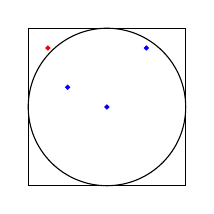
\begin{tikzpicture}
            \draw (-1, -1) -- (-1, 1) -- (1, 1) -- (1, -1) -- (-1, -1);
            \draw[blue, fill=blue] (0,0) circle (0.025cm);
            \draw[blue, fill=blue] (0.5, 0.75) circle (0.025cm);
            \draw[blue, fill=blue] (-0.5, 0.25) circle (0.025cm);
            \draw[red, fill=red] (-0.75, 0.75) circle (0.025cm);
            \draw (0,0) circle (1cm);
        \end{tikzpicture}

        \medskip
        \item $\Longrightarrow$ We can estimate the value of the constant $\pi$ by:
        
        \medskip
        \begin{itemize}
            \item Sampling points uniformly at random from the square
            
            \medskip
            \item Outputting the fraction of points inside the circle
        \end{itemize}
    \end{itemize}
\end{frame}

%

\begin{frame}{Monte Carlo method}
    \begin{itemize}
        \item Let $D : \Omega \rightarrow [0,1]$ be some \textcolor{blue}{probability distribution}.
    
        \medskip
        \item Let $f : \Omega \rightarrow \R_{\ge 0}$ be some \textcolor{blue}{function}.
        
        \medskip
        \item The goal is to estimate the \textcolor{blue}{expectation}
        
        \begin{equation*}
            \mu = \sum_{x\in\Omega} D(x) \cdot f(x)
        \end{equation*}

        \bigskip
        \item Draw $m$ independent samples $x_1,\ldots,x_m$ from $D$
            
        \medskip
        \item Output the empirical mean
        \begin{equation*}
            \hat{\mu} = \frac{1}{m} \sum_{x\in\Omega} f(x_i)
        \end{equation*}
    \end{itemize}
\end{frame}

%

\begin{frame}{Monte Carlo method}
    \begin{itemize}
        \item Define the \textcolor{blue}{second moment}
        
        \begin{equation*}
            \phi = \sum_{x\in\Omega} D(x) \cdot f(x)^2
        \end{equation*}
        
        \medskip
        \item 
        Define the \textcolor{blue}{relative variance} to be the ratio 
        
        \begin{equation*}
            \frac{\phi}{\mu^2}
        \end{equation*}
    \end{itemize}
\end{frame}

%

\begin{frame}{Classical Chebyshev inequality}
    \begin{itemize}
        \item Assume that $\frac{\phi}{\mu^2} \le B$ and set 
        
        \begin{equation*}
            m = O\left( \frac{B}{\varepsilon^2} \right)
        \end{equation*}
        
        \medskip
        \item \textcolor{blue}{Chebyshev inequality} implies that the empirical mean
        
        \begin{equation*}
            \hat{\mu} = \frac{1}{m} \sum_{i=1}^m f(x_i)
        \end{equation*}
        
        of the $m$ independent samples $x_1,\ldots,x_m$ from $D$ satisfies
        
        \begin{equation*}
            |\mu - \hat{\mu}| \le \varepsilon \cdot \mu
        \end{equation*}
        
        with probability $\ge \frac{3}{4}$.
    \end{itemize}
\end{frame}

%

\begin{frame}{Quantum samples}
    \begin{itemize}
    \item For a probability distribution $D$, define the corresponding \textcolor{blue}{quantum sample $|\psi_D\>$}
    
    \begin{equation*}
        |\psi_D\> = \sum_{x\in \Omega} \sqrt{D(x)} |x\>
    \end{equation*}
    
    \medskip
    \item Define the \textcolor{blue}{reflection $R_D$} around the quantum sample $|\psi_D\>$
    
    \begin{equation*}
        R_D = 2|\psi_D\>\<\psi_D| - I
    \end{equation*}
    \end{itemize}
    
\end{frame}

%

\begin{frame}{Quantum Chebyshev inequality}
    \begin{itemize}
        \item The quantum algorithm achieves a \textcolor{blue}{square root speed-up}:
    
        \medskip
        \begin{itemize}
            \item prepares a constant number of quantum samples $|\psi_D\>$
        
            \medskip
            \item invokes the reflection $R_D$
            \begin{equation*}
                O\left( \frac{\sqrt{B}}{\varepsilon} \right)
            \end{equation*}
            many times
            
            \medskip
            \item performs some other transformations (cost is smaller)
        \end{itemize}
        
        \bigskip
        \item The number of samples for the classical algorithm is
        \begin{equation*}
            O\left( \frac{B}{\varepsilon^2} \right) 
        \end{equation*}
    \end{itemize}
\end{frame}

%

\begin{frame}{Intuition behind quantum Chebyshev inequality}
\begin{itemize}
    \item Assume that values $f(x)$ are confined to the interval $[0, 1]$.
    
    \medskip
    \item Consider the \textcolor{blue}{quantum state $|\psi_{D,f}\>$} and the \textcolor{blue}{projector $P$}:
    \begin{align*}
        |\psi_{D,f}\> &= \sum_{x\in\Omega} \sqrt{D(x)} |x\> \otimes \left(
        \sqrt{f(x)} |1\> + \sqrt{1-f(x)} |0\> 
        \right) \\
        P &= I \otimes |1\>\<1|
    \end{align*}
    
    \medskip
    \item The desired mean $\mu=\sum_{x\in\Omega} D(x) \cdot f(x)$ is equal to
    \begin{equation*}
        \mu = \<\psi|P|\psi\>
    \end{equation*}
    
    \medskip
    \item $\Longrightarrow$ We can use \textcolor{blue}{amplitude estimation} in this special case.
    
    \medskip
    \item We handle general $f$ by decomposing $f$ as a weighted sum of functions with bounded output.
\end{itemize}
\end{frame}

%

\begin{frame}{Gibbs distribution}
    \begin{itemize}
        \item The partition function $Z(\beta)$ at inverse temperature is 
        \begin{equation*}
            Z(\beta) = \sum_{x\in\Omega} \exp\big( -\beta H(x) \big)
        \end{equation*}

        \item The \textcolor{blue}{Gibbs distribution $\pi_\beta$ at $\beta$} is a distribution on $\Omega$: 
        
        \medskip
        each state $x\in\Omega$ occurs with probability
        \begin{equation*}
            \pi_\beta(x) = \frac{\exp\big(-\beta H(x)\big)}{Z(\beta)}
        \end{equation*}

    \end{itemize}
\end{frame}

%

\begin{frame}{Estimating ratios of partition functions}
    \begin{itemize}
        \item Let $\beta$ and $\beta'$ be two inverse temperatures.
        
        \medskip
        \item Let $D$ be the Gibbs distribution $\pi_\beta$.
        
        \medskip
        \item Let $f$ be the function defined by
        \begin{equation*}
            f(x) = \exp\big( -(\beta'-\beta) H(x)\big)
        \end{equation*}
        
        \medskip
        \item The corresponding expectation $\mu$ is equal to
        \begin{equation*}
            \mu = \sum_{x\in \Omega} D(x) \cdot f(x) =
            \frac{Z(\beta')}{Z(\beta)}.
        \end{equation*}
        
        \item $\Longrightarrow$ We can \textcolor{blue}{estimate ratios of partition functions} provided that we can sample from Gibbs distributions.
    \end{itemize}
\end{frame}

%

\begin{frame}{Cooling schedule, telescoping product}
    \begin{itemize}
        \item We need to determine a suitable \textcolor{blue}{cooling schedule} $0=\beta_0 < \beta_1 < \ldots < \beta_\ell = \beta_{\max}$.
        
        \bigskip
        \item We can now express $Z(\beta_{\max})$ using the following \textcolor{blue}{telescoping product}:
        
        \begin{equation*}
            Z(\beta_{\max}) = 
            Z(\beta_0) \cdot
            \frac{Z(\beta_1)}{Z(\beta_0)} \cdot
            \frac{Z(\beta_2)}{Z(\beta_1)}
            \cdots 
            \frac{Z(\beta_\ell)}{Z(\beta_{\ell-1})}
        \end{equation*}
    \end{itemize}
\end{frame}

%

\begin{frame}{Previous approach based on product estimators}
    \begin{itemize}
        \item To estimate $Z(\beta_{\max})$, we
        
        \medskip
        \begin{itemize}
            \item \textcolor{blue}{estimate all ratios}
                \begin{equation*}
                    \frac{Z(\beta_{i+1})}{Z(\beta_{i})}
                \end{equation*} 
            with relative error $\varepsilon/\ell$ using quantum Chebyshev 
            
            \medskip
            \item \textcolor{blue}{take the product of the estimators}.
        \end{itemize}
        
        \bigskip
        \item This can be done efficiently provided that the \textcolor{red}{relative variances at all stages of the cooling schedule are small}.
    \end{itemize}
\end{frame}


%

\begin{frame}{New approach based on paired-product estimators}
    \begin{itemize}
        \item Let $\beta_i$ and $\beta_{i+1}$ be two adjacent inverse temperatures.
        
        \bigskip
        \item Let $m_i$ be the midpoint between $\beta_i$ and $\beta_{i+1}$.
        
        \bigskip
        \item Observe that the ratio $Z(\beta_{i+1}) / Z(\beta_i)$ 
        can be expressed as
        \begin{equation*}
            \frac{Z(\beta_{i+1})}{Z(m_i)}
            \, \cdot \,
            \left(
                \frac{Z(\beta_{i})}{Z(m_i)}
            \right)^{-1}
        \end{equation*}
    \end{itemize}
\end{frame}

%

\begin{frame}{New approach based on paired-product estimators}
\begin{itemize}
    \item We individually estimate 
        \begin{equation*}
            \frac{Z(\beta_{i+1})}{Z(m_i)} \quad\quad \mbox{and} \quad\quad
            \frac{Z(\beta_{i})}{Z(m_i)}
        \end{equation*}
    
    \bigskip
    \item We output their ratio as an estimate for $Z(\beta_{i+1})/Z(\beta_i)$.

    \bigskip
    \item This is highly beneficial because the \textcolor{blue}{resulting relative variances are significantly smaller} $\Rightarrow$ \textcolor{red}{fewer samples are required}.
\end{itemize}
    
\end{frame}

%

\begin{frame}{New approach based on paired-product estimators}
\begin{itemize}
    \item Moreover, the relative resulting variances depend on the overlap 
    \begin{align*}
        \<\pi_{\beta_i} | \pi_{\beta_{i+1}} \>
    \end{align*}
    
    between the quantum samples of the Gibbs distributions $\pi_{\beta_i}$ and $\pi_{\beta_{i+1}}$.
    
    \medskip
    \item This overlap can be estimated efficiently on a quantum computer.
    
    \medskip
    \item $\Longrightarrow$ We obtain a simple and efficient quantum algorithm for computing well-balanced cooling schedules.
\end{itemize}
    
\end{frame}

%

\begin{frame}{Markov chains}
\begin{itemize}
    \item \textcolor{blue}{Markov chains} make it possible to sample from complicated high-dimensional probability distributions.

    \medskip
    \item For instance, the \textcolor{blue}{Metropolis algorithm} is a method for constructing Markov chains that enable us to sample from \textcolor{blue}{Gibbs distributions}.
\end{itemize}
\end{frame}

%

\begin{frame}{Markov chains}
\begin{itemize}
    \item A Markov chain is described by a \textcolor{blue}{stochastic matrix $P=(p_{yx})$}.
    
    \medskip
    \item Let $x\in\Omega$ be the \textcolor{blue}{current} state.
    
    \medskip
    \item The \textcolor{blue}{transition probability $p_{yx}$} is the probability that the \textcolor{blue}{next} state is $y\in\Omega$.
    
\end{itemize}
\end{frame}

%

\begin{frame}{Mixing times of Markov chains}
\begin{itemize}
    \item $P$ has a \textcolor{blue}{limiting distribution $\pi$}.
    
    \medskip
    \item $\pi$ is the unique eigenvector corresponding to the largest eigenvalue $\lambda_1=1$ of $P$.

    \medskip
    \item The \textcolor{blue}{spectral gap $\Delta$} of $P$ is
    \begin{equation*}
        \Delta = 1 - \lambda_2(P)
    \end{equation*}
    where $\lambda_2$ denotes second largest eigenvalue of $P$.
    
    \medskip
    \item To obtain one sample from $\pi$, it suffices to perform
    \begin{equation*}
        O\left( \frac{1}{\Delta}\right)
    \end{equation*}
    transitions (independent of the initial state).
    
\end{itemize}

\end{frame}

%

\begin{frame}{Quantum Markov chains}
    \begin{itemize}
        \item We can construct a \textcolor{blue}{quantum Markov chain $U$}.
        
        \medskip
        \item $U$ is a unitary such that
        
        \medskip
        \begin{itemize}
            \item its unique eigenvector with eigenvalue $1$ (eigenphase $0$) is the \textcolor{blue}{quantum sample}
            \begin{equation*}
                |\psi_\pi\> = \sum_{x\in\Omega} \sqrt{\pi(x)} |x\>
            \end{equation*}
            
            \medskip
            \item all other eigenvectors have eigenphases that are at least
            \begin{equation*}
                \frac{1}{\sqrt{\Delta}}
            \end{equation*}
            away from $0$.
        \end{itemize}
    \end{itemize}
\end{frame}

%

\begin{frame}{Quantum Markov chains}
    \begin{itemize}
        \item We can implement the reflection 
        
        \begin{equation*}
            R_\pi = 2|\psi_\pi\>\<\psi_\pi|-I
        \end{equation*}
        by performing \textcolor{blue}{quantum phase estimation} of $U$.
        
        \medskip
        \item We have to invoke the unitary $U$
        \begin{equation*}
            O\left(
            \frac{1}{\sqrt{\Delta}}
            \right)
        \end{equation*}
        times to implement $R_\pi$.
        
        \medskip
        \item We have to invoke the stochastic matrix $P$
        \begin{equation*}
            O\left(
            \frac{1}{\Delta}
            \right)
        \end{equation*}
        times to obtain a sample from limiting distribution $\pi$.
    \end{itemize}
\end{frame}

%

\end{document}

%%%%%%%%%%%%%%%%%%%%%%%%%%%%%%%%%%%%%%%%%%%%%%%%%%%%%%%%%%%%%%%%%%%%%%%%%%%%%%%%%%%%%%%%%%%%%%%%%%%%%%%%%%%%%

% optional slides

\begin{frame}{Complexity of Hamiltonians}
    \begin{itemize}
        \item Finding low energy states is NP-hard.
        
        \medskip
        \item Counting low energy states is \#P-hard.
    \end{itemize}
\end{frame}

%

\begin{frame}{Complexity of Hamiltonians}
    \begin{itemize}
        \item For instance, consider some Boolean formula 
        \begin{equation*}
            \phi : \{0,1\}^m \rightarrow \{0,1\}, \quad
            \phi = C_1 \land C_2 \land \ldots \land C_n
        \end{equation*} 
        in conjunctive normal form.
        
        \medskip
        \item Let $\Omega=\{0,1\}^m$ and $H : \Omega \rightarrow \{0,1,\ldots,n\}$.
        
        \medskip 
        \item Define the energy $H(x)$ of a truth-value assignment $x\in\Omega$ to be the number of clauses that are violated by $x$.
    \end{itemize}
\end{frame}

\end{document}


%%%%%%%%%%%%%%%%%%%%%%%%%%%%%

Abstract:

We consider the problem of approximating the partition function of a classical Hamiltonian using simulated annealing. This requires the computation of a cooling schedule, and the ability to estimate the mean of the Gibbs distributions at the corresponding inverse temperatures. We propose classical and quantum algorithms for these two tasks, achieving two goals: (i) we simplify the seminal work of Štefankovič, Vempala and Vigoda (J. ACM, 56(3), 2009), improving their running time and almost matching that of the current classical state of the art; (ii) we quantize our new simple algorithm, improving upon the best known algorithm for computing partition functions of many problems, due to Harrow and Wei (SODA 2020). A key ingredient of our method is the paired-product estimator of Huber (Ann. Appl. Probab., 25(2), 2015). The proposed quantum algorithm has two advantages over the classical algorithm: it has quadratically faster dependence on the spectral gap of the Markov chains as well as the precision, and it computes a shorter cooling schedule, which matches the length conjectured to be optimal by Štefankovič, Vempala and Vigoda.

Joint work with Srinivasan Arunachalam, Vojtech Havlicek, Giacomo Nannicini, Kristan Temme,
https://arxiv.org/abs/2009.11270